\section{Atividades}

Identificar Associações de Resistores em Paralelo e em Série.


\begin{minipage}{\linewidth}
  \centering
  \begin{minipage}{0.45\linewidth}
    \begin{figure}[H]
      \centering
      \label{fig:ativ1}
      \caption{Circuito 1}
      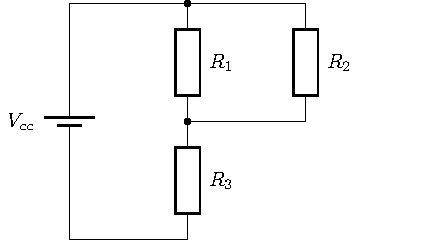
\includegraphics[scale=1.0]{fig-ativ1}
    \end{figure}
  \end{minipage}
  \hspace{0.05\linewidth}
  \begin{minipage}{0.45\linewidth}
    \begin{figure}[H]
      \centering
      \label{fig:ativ2}
      \caption{Circuito 2}
      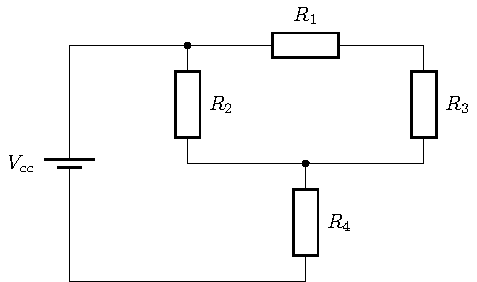
\includegraphics[scale=1.0]{fig-ativ2}
    \end{figure}
  \end{minipage}
\end{minipage}

\begin{minipage}{\linewidth}
  \centering
  \begin{minipage}{0.45\linewidth}
    \begin{figure}[H]
      \centering
      \label{fig:ativ3}
      \caption{Circuito 3}
      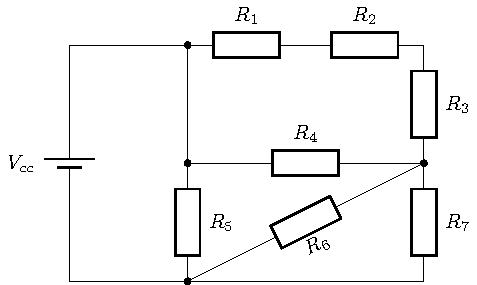
\includegraphics[scale=1.0]{fig-ativ3}
    \end{figure}
  \end{minipage}
  \hspace{0.05\linewidth}
  \begin{minipage}{0.45\linewidth}
    \begin{figure}[H]
      \centering
      \label{fig:ativ4}
      \caption{Circuito 4}
      \includegraphics[scale=1.0]{fig-ativ4}
    \end{figure}
  \end{minipage}
\end{minipage}
